\section{Results}
\subsection{Description of data analysis} \label{sec:stoc_descr}
The first goal of this model has been to reproduce the main results in \autocite{Huisman2002HowPersist}, then some original work has been produced concerning different boundary conditions.
A first analysis which can be performed is qualitative and concerns the depth profile of the phytoplankton population. Another, more quantitative analysis results by evaluating the occurrence or absence of a bloom depending on the set of parameters chosen, in the same way as shown in \autoref{fig:huisman_Dzplot}. The simplest approach to the problem would be to look at the population averaged in time when a steady-state is reached; however this condition has been reached only for a part of the parameters set explored ($\mathcal{P}$), due to the high computation time needed 
\footnote{%As it is explained in \autoref{sec:stoc_numerical_details}, t 
The time step goes linearly with the inverse of $D$, which spans over many orders, thus increasing by orders the total time of computation keeping fixed the characteristic time.}. This subset will be called $\mathcal{S}$ from now on.
In particular, in the no-bloom zone the number of particles should go to zero, a condition which occurs only at the steady-state, by definition.
Even if proper result can be obtained only for a subset of parameters, a way has been attempted to give sense to the whole set. First, the analysis is limited to the subset $\mathcal{S}$: if the steady-state results present an analogous behaviour to the partial results, then all the results obtained before the steady-state is reached can be expected to give meaningful results
\footnote{The whole process is somehow arbitrary, but with "analogous behaviour" one could mean a trend in significantly higher or lower values of the final population.}. However, it is important to stress that this results are not rigorous and this approach should be intended as exploratory: estimates for critical values of $D$ and $z$ will be given only when internal to the subset $\mathcal{S}$.

\subsection{Reflective bottom} \label{sec:stoc_refl}
Imposing boundary reflective conditions on both the top and the bottom of the interval corresponds to a mixed layer as tall as the column of water, and matches the hypotheses made in \autocite{Huisman2002HowPersist}. Although not realistic, these conditions allow in this way the comparison with previous models, which can validate the results obtained if equivalent. 

In \autoref{img:stoc_refl_depth_profiles_cfr} and \autoref{fig:stoc_res_profiles_z20} the depth profiles are shown for \autocite{Huisman2002HowPersist} and the model here developed, for different combination of parameters: an exact correspondence is not to be expected, since the two models are different (see \autoref{sec:peculiar_1D}), but the qualitative comparison results in a succesful reproduction of all the features of \autocite{Huisman2002HowPersist}.

\begin{figure} 
    \centering
    \begin{subfigure}[b]{0.3\textwidth}
        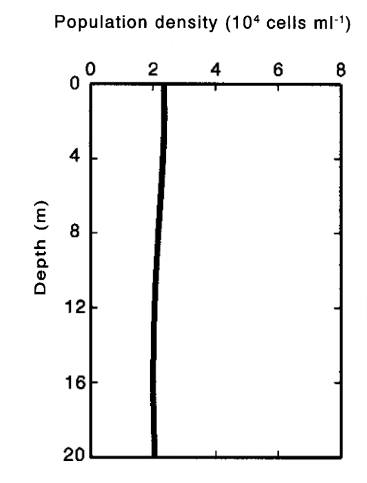
\includegraphics[width=\textwidth]{img/H_dep_prof_d-1}
        \caption{}
        \label{fig:huism_prof_d-1}
    \end{subfigure}
    \begin{subfigure}[b]{0.3\textwidth}
        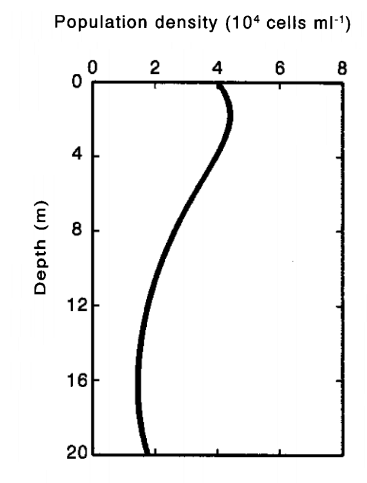
\includegraphics[width=\textwidth]{img/H_dep_prof_d0}
        \caption{}
        \label{fig:huism_prof_d0}
    \end{subfigure}
    \begin{subfigure}[b]{0.3\textwidth}
        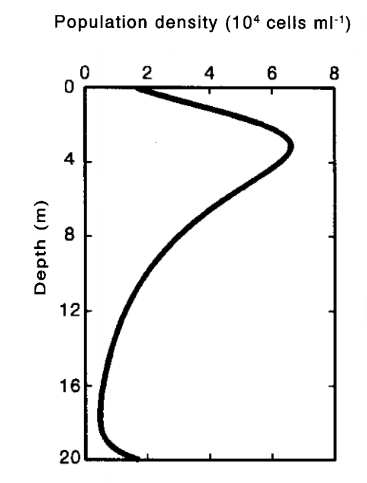
\includegraphics[width=\textwidth]{img/H_dep_prof_d1}
        \caption{}
        \label{fig:huism_prof_d1}
    \end{subfigure}
    \caption{Comparison between the depth profiles obtained in \autocite{Huisman2002HowPersist}. The varying parameter is the effective diffusivity: \autoref{fig:huism_prof_d-1}, \(D=0.036m/s^2\); \autoref{fig:huism_prof_d0}), \(D=0.36m/s^2\); \autoref{fig:huism_prof_d1}, \(D=3.6m/s^2\).}
    \label{img:stoc_refl_depth_profiles_cfr}
\end{figure}
 
\begin{figure}
    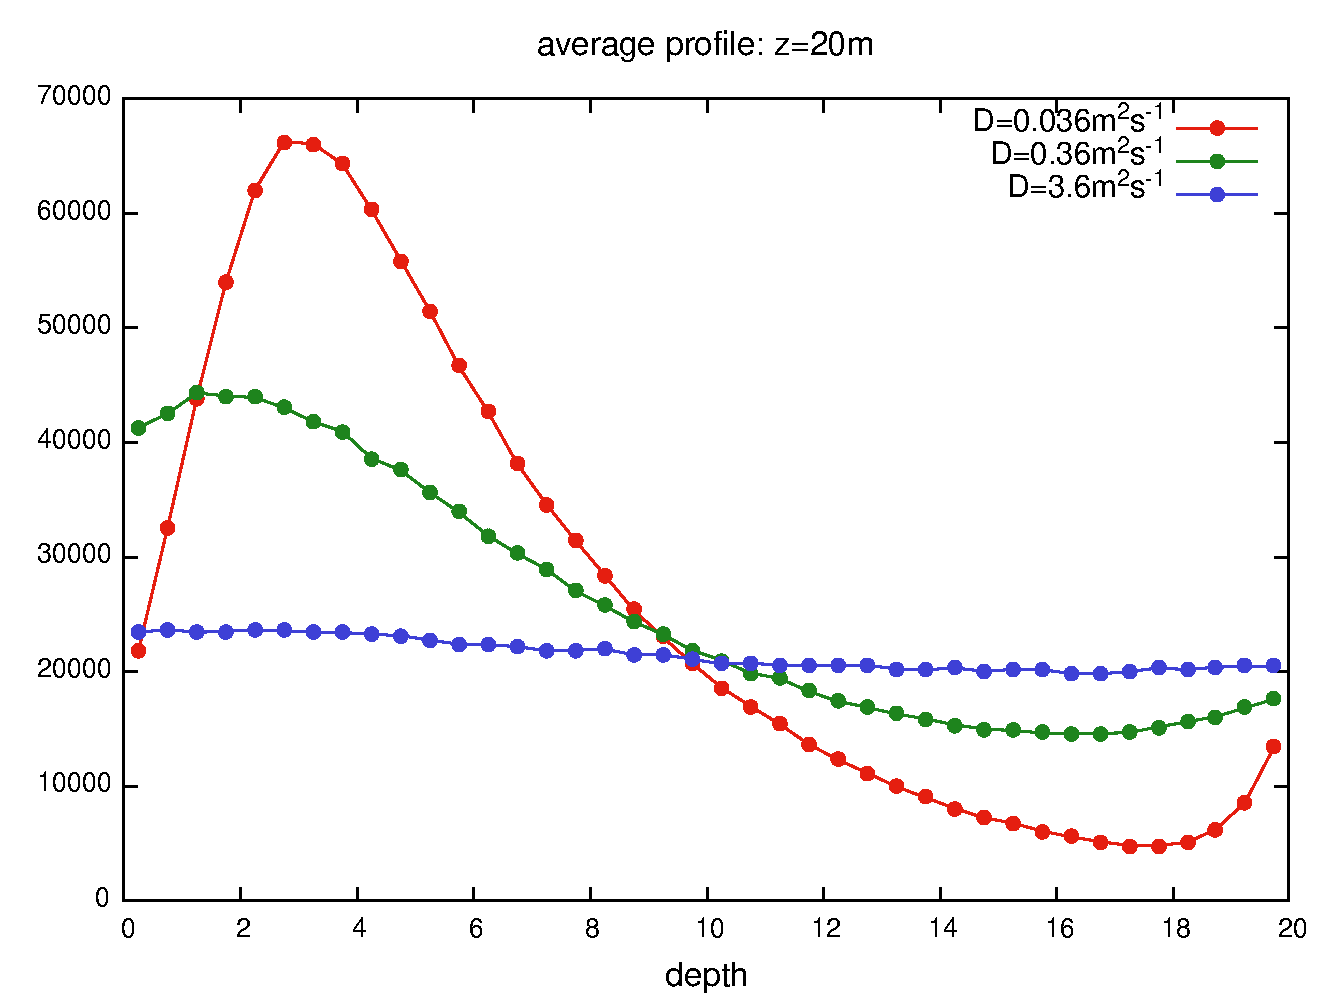
\includegraphics[width=\textwidth]{data/1D_model/reflective_bottom/profiles_z_20}
    \caption{Depth profiles with the same parameters as \autoref{fig:huism_prof_d1}, for comparison; the shape is qualitatively the same, while the normalization changes due to the different number of particles simulated.}
    \label{fig:stoc_res_profiles_z20}
\end{figure}
 

In order to determine the conditions which favour a bloom, the method described in \autoref{sec:stoc_descr} has been used. First, the subset $\mathcal{S}$ of the parameters space for which simulations have reached the steady-state is considered: a plot of this subset is shown in \autoref{fig:stoc_subset_steady_pop}. The population has been averaged in time, once the steady-state has been reached, in order to reduce the random fluctuation introduced with a stochastic model. The points expected to have no bloom actually reach a null population.

\begin{figure} 
  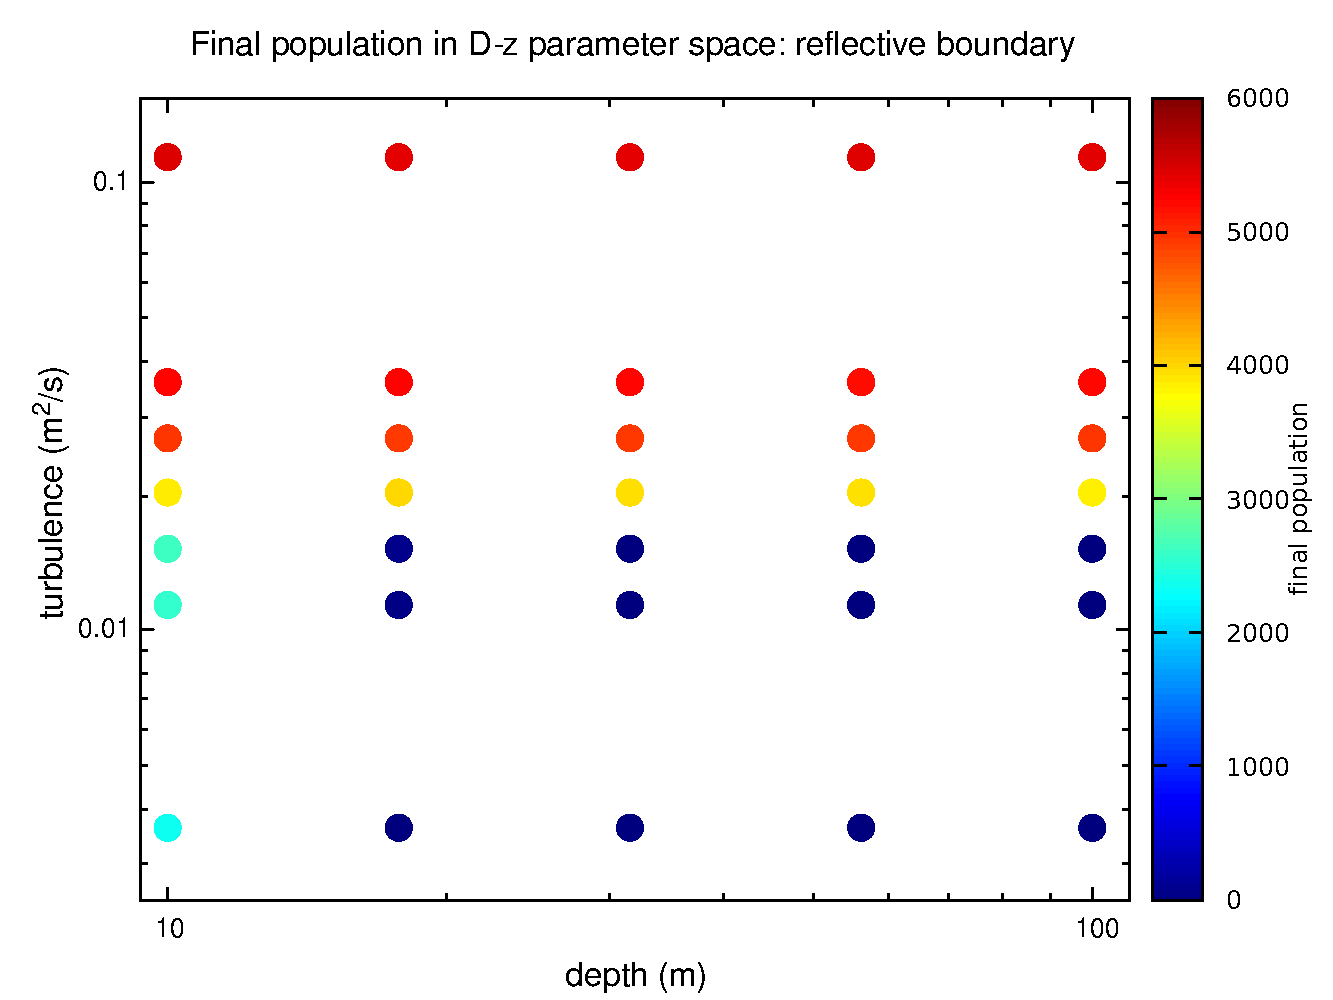
\includegraphics[width=0.9\textwidth]{data/1D_model/reflective_bottom/bottom_right/bloom_pop}
  \caption{Final population in the subset of parameter space for which the steady-state has been reached: the colour scale refers to the number of particle averaged in time. The points in the lower part of the scale are actually zero, meaning the complete death of the population.}
    \label{fig:stoc_subset_steady_pop}
\end{figure}

In \autoref{fig:stoc_subset_steady_pop_zoom}, more simulations have been run for the parameters around the critical values, in order to compare them with the results. Both the compensation depth and the minimum diffusivity are near the values predicted in \autoref{sec:huism_crit_parameters}, but while for $z$ the simulations show accordance up to the resolution considered, for $D$ a discrepancy is noticeable. This discrepancy may be due to the different numerical implementation of the code, in addition to the stochastic approach used here, instead of using a deterministic equation. The result is however satisfactory, when looking at the many orders of magnitude spanned in the simulations, considering that the result differ from what was expected by less than 30\%.

\begin{figure} 
    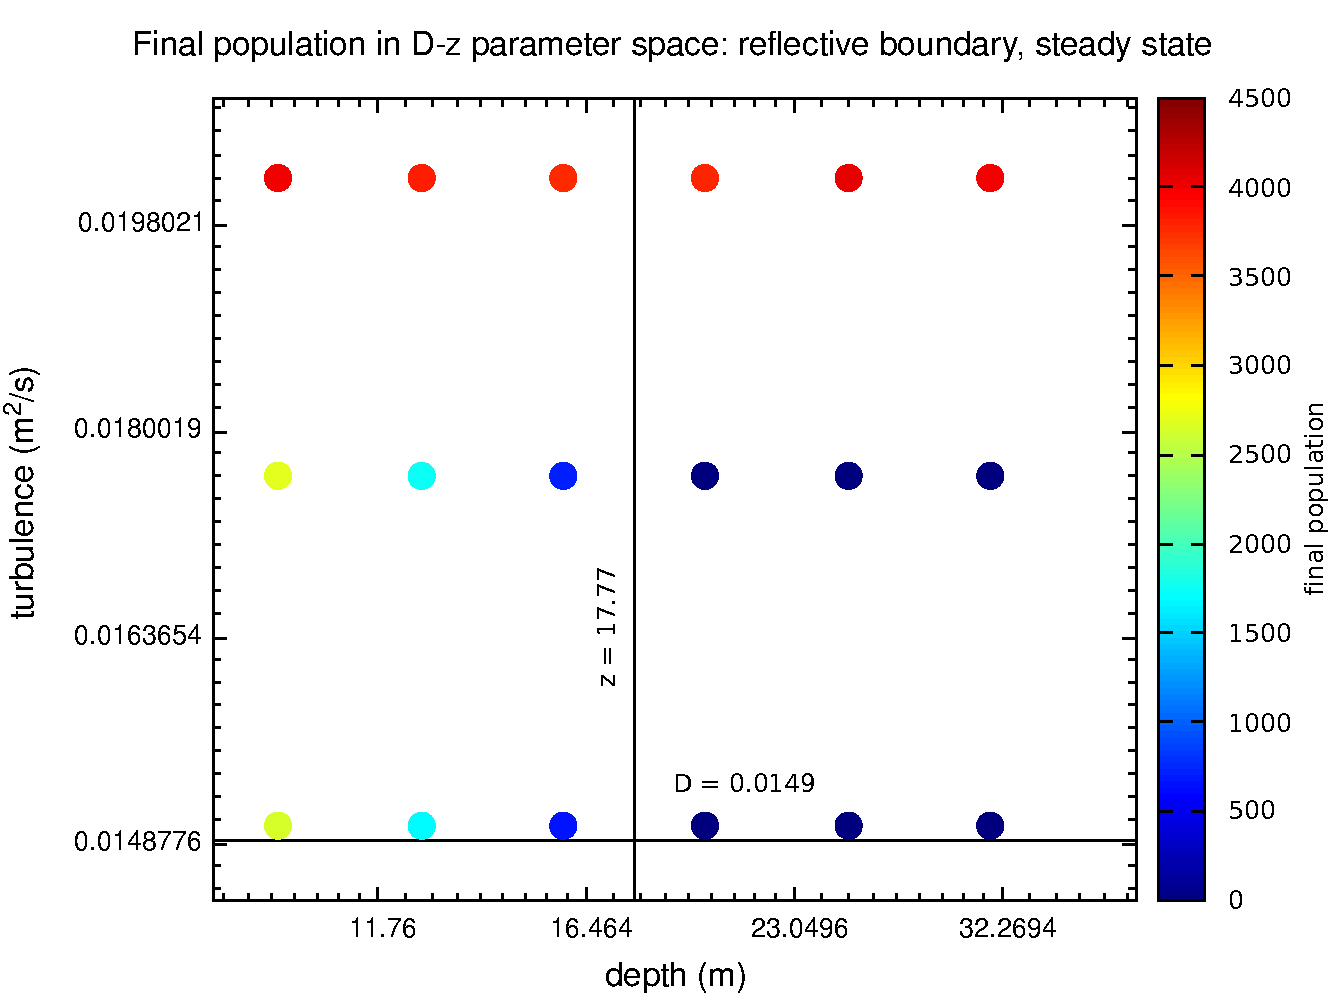
\includegraphics[width=0.9\textwidth]{data/1D_model/reflective_bottom/bottom_right_zoom/bloom_pop}
    \caption{Final population in a restricted area of the parameter space, in order to estimate the critical values ($D_min$ and $z_c$, see \autoref{sec:huism_crit_parameters}), which are represented by two solid lines.}
    \label{fig:stoc_subset_steady_pop_zoom}
\end{figure}

Coming to the wider set of parameters considered in \autocite{Huisman2002HowPersist}, as said in \autoref{sec:stoc_descr} the code required too much computational time to reach the steady-state in every point. The meaning of \autoref{fig:stoc_refl_all_pop} is thus not a rigorous analysis, while a qualitative trend can be identified which agrees with the reference model. 

\begin{figure} 
  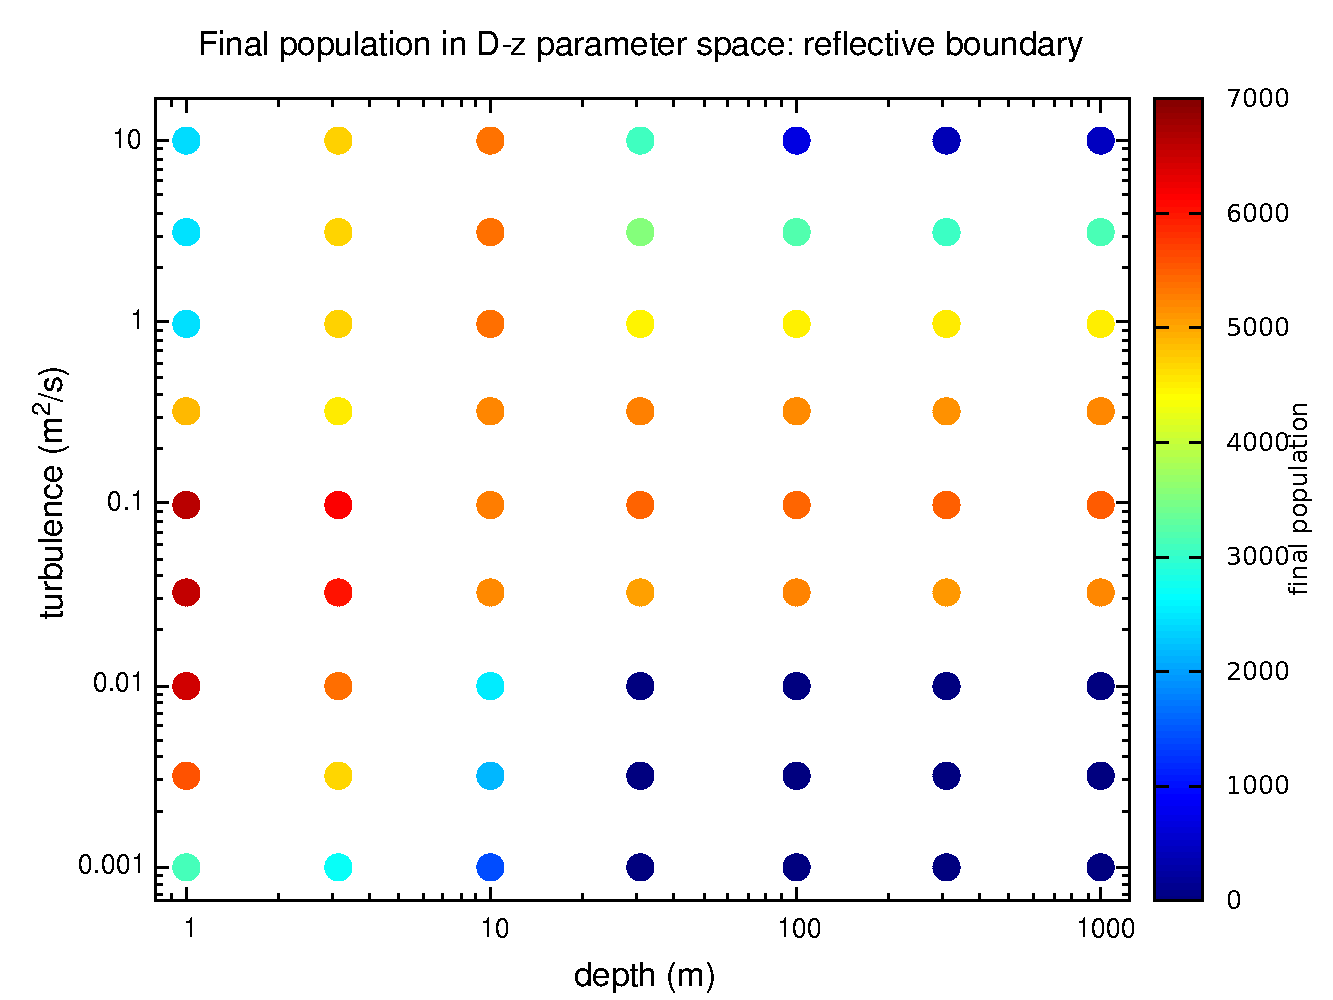
\includegraphics[width=\textwidth]{data/1D_model/reflective_bottom/global/bloom_pop}
  \caption{The plot shows the final populations for the point in the parameters space D-z.}
  \label{fig:stoc_refl_all_pop}
\end{figure}

\subsection{Absorbing bottom} \label{sec:stoc_res_abs}
After reproducing the results of \autocite{Huisman2002HowPersist} in \autoref{sec:stoc_refl}, other unexplored conditions have been considered, substituting the reflective conditions at the bottom with absorbing ones, i.e. when a particle reaches the bottom it is killed and removed from the simulation \footnote{This also applies when a particle is created over the border, which happens during reproduction, when the position of new particle is slightly randomized to avoid putting it on the same flow-line. % (see \autoref{sec:stoc_reproduction}).
}.


 \label{sec:stoc_res_profile}
The profiles are overall similar to the ones obtained when imposing reflective conditions, since the bulk behaviour prevails; the main difference concerns the accumulation at the bottom, present in \autoref{fig:stoc_res_profiles_z20} and absent here, this fact due to the particles removal at the bottom. An example is shown in \autoref{fig:stoc_abs_profile}, the number of particles goes to zero towards the bottom, as expected.

\begin{figure} 
  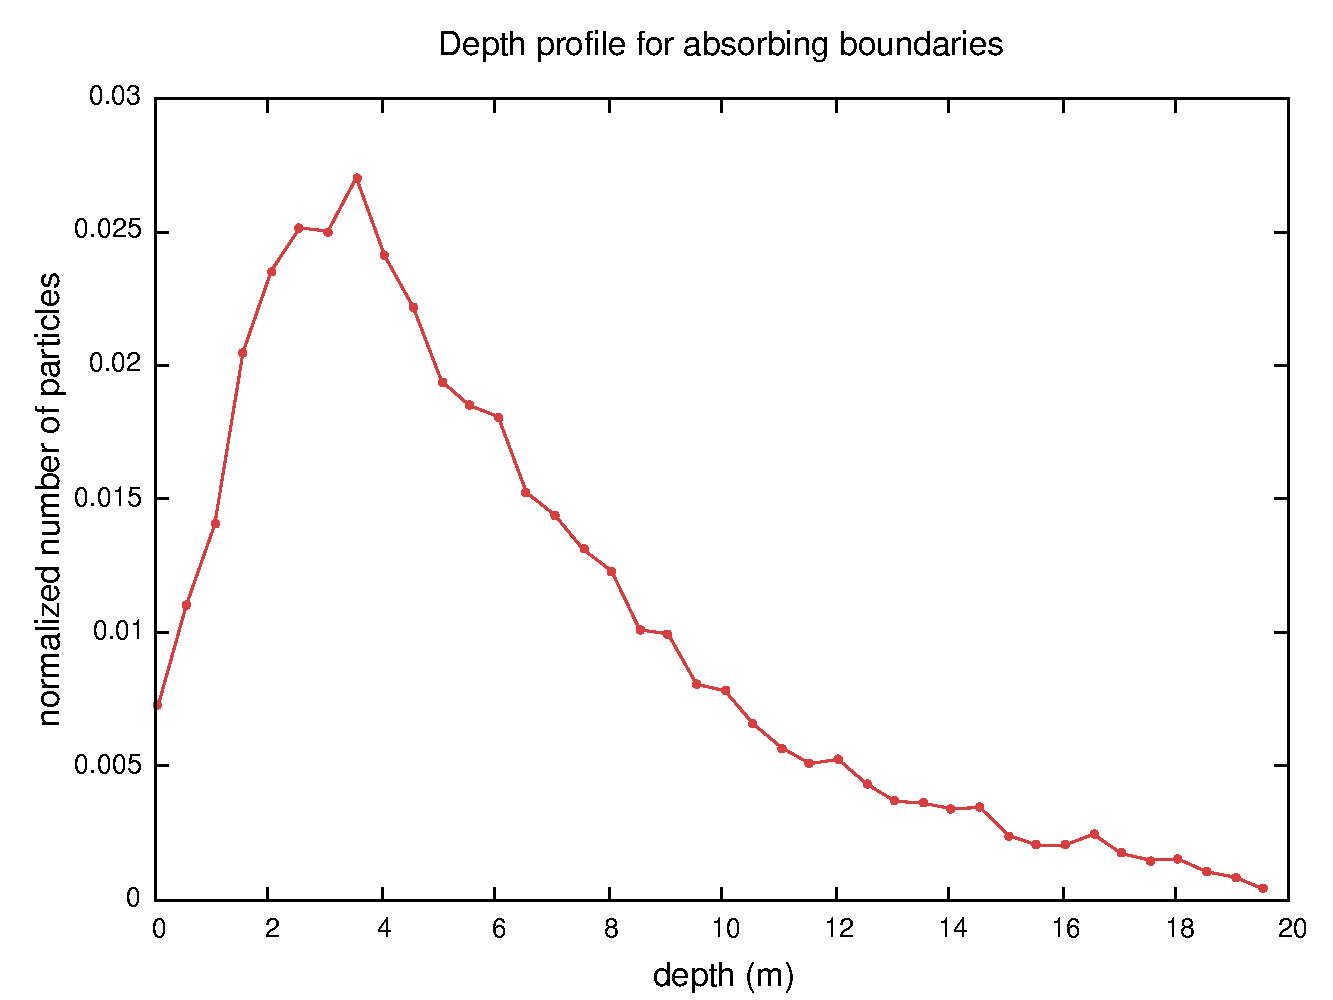
\includegraphics[width=\textwidth]{data/1D_model/absorbing_bottom/abs_sample_profile}
  \caption{A sample depth profile with absorbing conditions ($z=20m$,$D=3.6\cdot10^{-2}m^2h^{-1}$).}
  \label{fig:stoc_abs_profile}
\end{figure}

%\begin{figure} 
%  \centering
%  \begin{subfigure}[b]{0.4\textwidth}
%    \includegraphics[width=0.4\textwidth]{prg/numerical_1D/stoc_fin_diff_oop/sample_profiles/analysis/dep_prof_d-1}
%    \caption{}
%  \end{subfigure}
%
%  \begin{subfigure}[b]{0.4\textwidth}
%    \includegraphics[width=0.4\textwidth]{prg/numerical_1D/stoc_fin_diff_oop/sample_profiles/analysis/dep_prof_d0}
%    \caption{}
%  \end{subfigure}
%
%  \begin{subfigure}[b]{0.4\textwidth}
%    \includegraphics[width=0.4\textwidth]{prg/numerical_1D/stoc_fin_diff_oop/sample_profiles/analysis/dep_prof_d1}
%    \caption{}
%  \end{subfigure}
%
%  \caption{Depth profiles obtained with boundary conditions at the bottom. The varying parameter is the effective diffusivity: (a),(b) \(D=0.36\cdot10^{-1}m/s^2\); (c),(d) \(D=0.36m/s^2\); (e),(f) \(D=3.6m/s^2\).}
%  \label{img:stoc_abs_depth_profiles_cfr}
%\end{figure}

The blooming pattern resulting from the simulation is shown in \autoref{fig:stoc_abs_all_pop}. On the right side of the plot, the results are essentially analogous to the ones obtained in reflective conditions, while on the left side, at low depths, no bloom is present. This fact is easily explained considering that with the same parameters, but reflective conditions, the peak of the distribution lies at the bottom of the water column, while now they cannot accumulate, because they are removed when they get there.

\begin{figure} 
  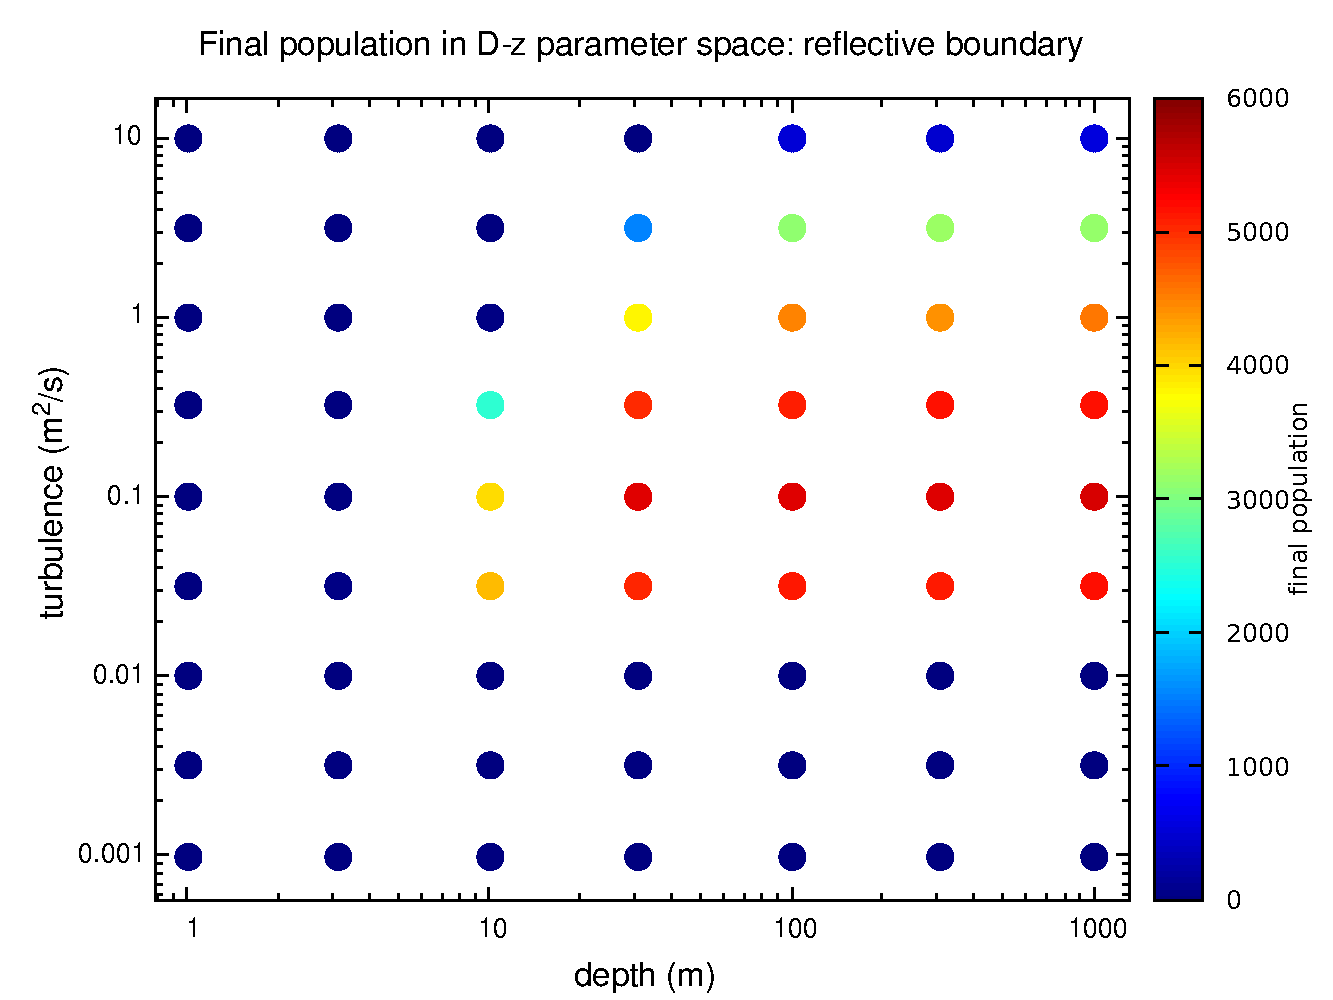
\includegraphics[width=\textwidth]{data/1D_model/absorbing_bottom/bloom_pop}
  \caption{The plot shows the final populations for the points in the parameters space D-z, with absorbing boundary conditions at the bottom.}
  \label{fig:stoc_abs_all_pop}
\end{figure}

